\section{Problem set 3}
\subsection{Preface}

The goal of this problem set was brief introduction to work with IrDA transmission
and how oscilloscope works.

\subsection{Assignment}

I've received two \texttt{logicdata} files with data from some remote in binary form via email from the lecturer.

\subsubsection{Analysis}

For the analysis of the program I've used two tools. First of them, ,,Saleae Logic'', has some built in protocol analyzers, but none of them was sufficient. I've analyzed the source with ,,Async Serial'' on channel 2, but it only detected many similar repeating sequences of bits \texttt{0b 1110 0000} and some data errors.

The next attempt to analyze the signal was done using ,,PulseView'' program. To prepare data to analyze it using ,,PulseView'' I had to extract data from \texttt{logicdata} format to raw binary data. In next step I've importet raw binary data to ,,PulseView'' and analyzed the data using built-in analyzers - \texttt{RC-5} and \texttt{NEC}. For the \texttt{RC-5} analyzer, program didn't find anything valid. For the \texttt{NEC} analyzer, the result was positive. Thanks to that program I've concluded that the protocol used to emit the analyzed signal was \texttt{NEC}. Figure \ref{fig:nec-pulse-view} contains screen from ,,PulseView'' with protocol detected by the program. As it can be seen there, the decoded part of signal contains \texttt{Leader code}, two bytes of address and two bytes of command, as it is in the \texttt{NEC} protocol.

\begin{figure}[!htb]
  \center{
    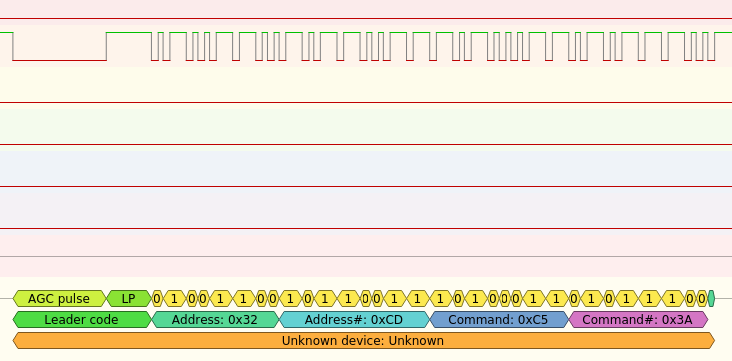
\includegraphics[scale=0.4]{drawings/nec}
    \caption{\label{fig:nec-pulse-view}} Screen from ,,PulseView'' program after applying \texttt{IR NEC} decoder on raw data from logicdata.}
\end{figure}

\subsubsection{Retransmitter}

To create retransmitter I've created a simple Arduino program using IR receiver and IR diode. Basic idea behind the program is to, first of all, receive the transmitted \texttt{NEC} signal using IR diode - for this case, the \texttt{IRrecv} class of \texttt{IRRemote} library was used. For every received 32 bits of data, a \texttt{NEC} protocol frame was created and resend using \texttt{IRsend.sendNEC} method.
